The field was discretized in equally sized squares of $50 \times 50 cm$ for a total of $K=36$ states.  
 
 \begin{figure}[H]
 \centering
  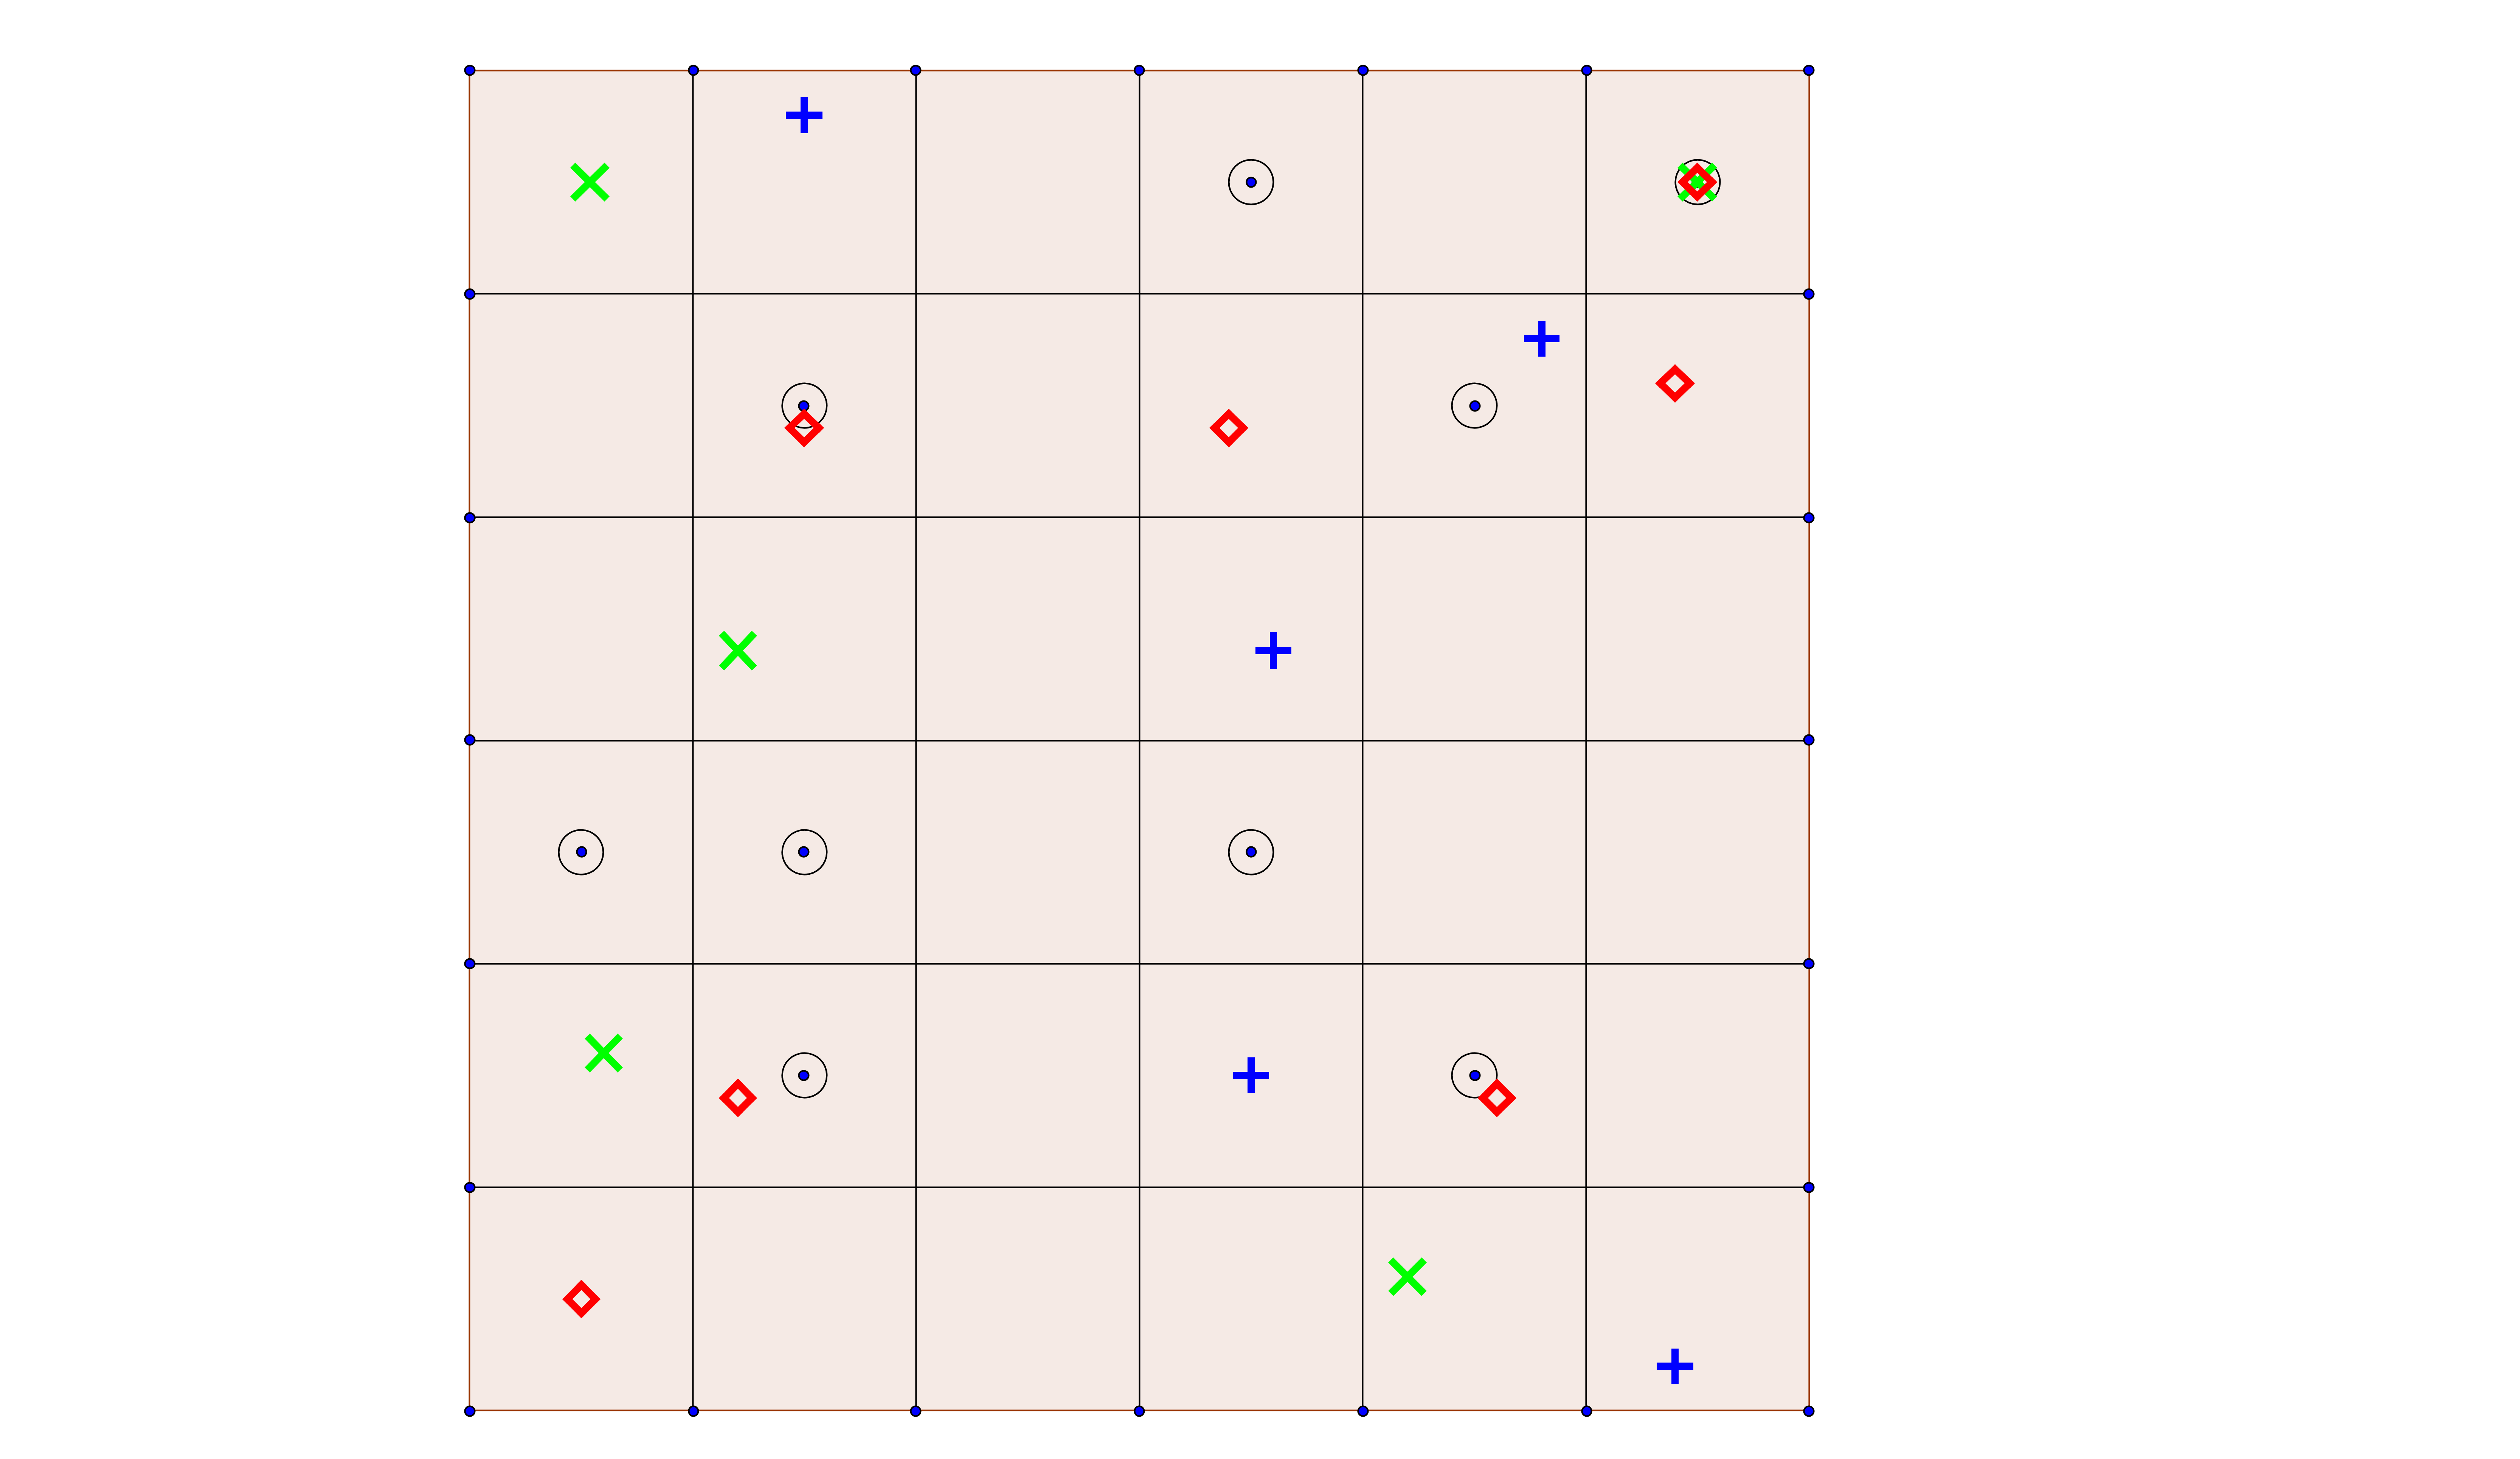
\includegraphics[width = 0.8\textwidth]{hw3_map.png}
  \caption{The discretized field}
  \end{figure}

The regions are defined as: $R_i$ for $i\in \{1,..,36\}$


 The transition system is a tuple in the form:
$\mathcal{T}=(S,S_0,\sum,\rightarrow,\Pi,\mathcal{L})$\\
The defined states $S=\{R_1,R_2,...R_{36}\}.$\\
$\Pi=\{R,G,B,O\}$\\
The corresponding labels:\\
$\mathcal{L}(R_1)=\{R\}$\\
$\mathcal{L}(R_2)=\{G\}$\\
$\mathcal{L}(R_3)=\{O\}$\\
$\mathcal{L}(R_4)=\{\}$\\
$\mathcal{L}(R_5)=\{\}$\\
$\mathcal{L}(R_6)=\{G\}$\\
$\mathcal{L}(R_7)=\{B\}$\\
$\mathcal{L}(R_8)=\{R,O\}$\\
$\mathcal{L}(R_9)=\{G\}$\\
$\mathcal{L}(R_{10})=\{O\}$\\
$\mathcal{L}(R_{11})=\{R,O\}$\\
$\mathcal{L}(R_{12})=\{\}$\\
$\mathcal{L}(R_{13})=\{\}$\\
$\mathcal{L}(R_{14})=\{\}$\\
$\mathcal{L}(R_{15})=\{\}$\\
$\mathcal{L}(R_{16})=\{\}$\\
$\mathcal{L}(R_{17})=\{\}$\\
$\mathcal{L}(R_{18})=\{\}$\\
$\mathcal{L}(R_{19})=\{O\}$\\
$\mathcal{L}(R_{20})=\{R\}$\\
$\mathcal{L}(R_{21})=\{B\}$\\
$\mathcal{L}(R_{22})=\{O\}$\\
$\mathcal{L}(R_{23})=\{B\}$\\
$\mathcal{L}(R_{24})=\{\}$\\
$\mathcal{L}(R_{25})=\{\}$\\
$\mathcal{L}(R_{26})=\{B,O\}$\\
$\mathcal{L}(R_{27})=\{\}$\\
$\mathcal{L}(R_{28})=\{\}$\\
$\mathcal{L}(R_{29})=\{R,O\}$\\
$\mathcal{L}(R_{30})=\{G\}$\\
$\mathcal{L}(R_{31})=\{R,G\}$\\
$\mathcal{L}(R_{32})=\{R\}$\\
$\mathcal{L}(R_{33})=\{\}$\\
$\mathcal{L}(R_{34})=\{\}$\\
$\mathcal{L}(R_{35})=\{\}$\\
$\mathcal{L}(R_{36})=\{B\}$\\

The actions:
$\sum=\{N,S,W,E\}$.\\
The transitions can be seen in figure \ref{fig:INT}. 
%a_N-North (up), a_S=south (down), a_W-west (left), a_E-east (right)
%adds transition image
\begin{figure}[H]
    \centering

    \begin{tikzpicture}[-latex ,auto ,node distance =2 cm and 2cm  ,semithick ,state/.style ={ circle ,top color =white , bottom color =blue ,draw,blue , text=black , minimum width =1 cm}]
    \node[state,initial ,initial where=left,] (R_6)   {$q_\text{start}$};
    
    \node[state] (R_6) {$R_6$};
    \node[state] (R_5) [below of=R_6] {$R_5$};
    \node[state] (R_4) [below of=R_5] {$R_4$};
    \node[state] (R_3) [below of=R_4] {$R_3$};
    \node[state] (R_2) [below of=R_3] {$R_2$};
    \node[state] (R_1) [below of=R_2] {$R_1$};
    
    \node[state] (R_7) [right of=R_6] {$R_7$};
    \node[state] (R_8) [below of=R_7] {$R_8$};
    \node[state] (R_9) [below of=R_8] {$R_9$};
    \node[state] (R_10) [below of=R_9] {$R_{10}$};
    \node[state] (R_11) [below of=R_10] {$R_{11}$};
    \node[state] (R_12) [below of=R_11] {$R_{12}$};

    \node[state] (R_18) [right of=R_7] {$R_{18}$};
    \node[state] (R_17) [below of=R_18] {$R_{17}$};
    \node[state] (R_16) [below of=R_17] {$R_{16}$};
    \node[state] (R_15) [below of=R_16] {$R_{15}$};
    \node[state] (R_14) [below of=R_15] {$R_{14}$};
    \node[state] (R_13) [below of=R_14] {$R_{13}$};
    
    \node[state] (R_19) [right of=R_18] {$R_{19}$};
    \node[state] (R_20) [below of=R_19] {$R_{20}$};
    \node[state] (R_21) [below of=R_20] {$R_{21}$};
    \node[state] (R_22) [below of=R_21] {$R_{22}$};
    \node[state] (R_23) [below of=R_22] {$R_{23}$};
    \node[state] (R_24) [below of=R_23] {$R_{24}$};

    \node[state] (R_30) [right of=R_19] {$R_{30}$};
    \node[state] (R_29) [below of=R_30] {$R_{29}$};
    \node[state] (R_28) [below of=R_29] {$R_{28}$};
    \node[state] (R_27) [below of=R_28] {$R_{27}$};
    \node[state] (R_26) [below of=R_27] {$R_{26}$};
    \node[state] (R_25) [below of=R_26] {$R_{25}$};
    
    \node[state] (R_31) [right of=R_30] {$R_{31}$};
    \node[state] (R_32) [below of=R_31] {$R_{32}$};
    \node[state] (R_33) [below of=R_32] {$R_{33}$};
    \node[state] (R_34) [below of=R_33] {$R_{34}$};
    \node[state] (R_35) [below of=R_34] {$R_{35}$};
    \node[state] (R_36) [below of=R_35] {$R_{36}$};
%paths
    \path (R_1) edge [bend left] node {$N$} (R_2);
    \path (R_1) edge [bend left] node {$E$} (R_12);
    
    \path (R_2) edge [bend left] node {$N$} (R_3);
    \path (R_2) edge [bend left] node {$E$} (R_11);
    \path (R_2) edge [bend left] node {$S$} (R_1);
    
    \path (R_3) edge [bend left] node {$N$} (R_4);
    \path (R_3) edge [bend left] node {$E$} (R_10);
    \path (R_3) edge [bend left] node {$S$} (R_2);

    
    \path (R_4) edge [bend left] node {$N$} (R_5);
    \path (R_4) edge [bend left] node {$E$} (R_9);
    \path (R_4) edge [bend left] node {$S$} (R_3);
    
    \path (R_5) edge [bend left] node {$N$} (R_6);
    \path (R_5) edge [bend left] node {$E$} (R_8);
    \path (R_5) edge [bend left] node {$S$} (R_4);
    
    \path (R_6) edge [bend left] node {$E$} (R_7);
    \path (R_6) edge [bend left] node {$S$} (R_5);
    
    \path (R_7) edge [bend left] node {$S$} (R_8);
    \path (R_7) edge [bend left] node {$E$} (R_18);
    \path (R_7) edge [bend left] node {$W$} (R_6);
    
    \path (R_8) edge [bend left] node {$N$} (R_7);
    \path (R_8) edge [bend left] node {$S$} (R_9);
    \path (R_8) edge [bend left] node {$E$} (R_17);
    \path (R_8) edge [bend left] node {$W$} (R_5);
    
    \path (R_9) edge [bend left] node {$N$} (R_8);
    \path (R_9) edge [bend left] node {$S$} (R_10);
    \path (R_9) edge [bend left] node {$E$} (R_16);
    \path (R_9) edge [bend left] node {$W$} (R_4);
    
    \path (R_10) edge [bend left] node {$N$} (R_9);
    \path (R_10) edge [bend left] node {$S$} (R_11);
    \path (R_10) edge [bend left] node {$E$} (R_15);
    \path (R_10) edge [bend left] node {$W$} (R_3);
    
    \path (R_11) edge [bend left] node {$N$} (R_10);
    \path (R_11) edge [bend left] node {$S$} (R_12);
    \path (R_11) edge [bend left] node {$E$} (R_14);
    \path (R_11) edge [bend left] node {$W$} (R_2);
    
    \path (R_12) edge [bend left] node {$N$} (R_11);
    \path (R_12) edge [bend left] node {$E$} (R_13);
    \path (R_12) edge [bend left] node {$W$} (R_1);
    
    \path (R_13) edge [bend left] node {$N$} (R_14);
    \path (R_13) edge [bend left] node {$W$} (R_12);
    \path (R_13) edge [bend left] node {$E$} (R_24);
    
    \path (R_14) edge [bend left] node {$S$} (R_13);
    \path (R_14) edge [bend left] node {$N$} (R_15);
    \path (R_14) edge [bend left] node {$W$} (R_11);
    \path (R_14) edge [bend left] node {$E$} (R_23);
    
    \path (R_15) edge [bend left] node {$N$} (R_16);
    \path (R_15) edge [bend left] node {$S$} (R_14);
    \path (R_15) edge [bend left] node {$E$} (R_22);
    \path (R_15) edge [bend left] node {$W$} (R_10);
    
\path (R_16) edge [bend left] node {$N$} (R_17);
    \path (R_16) edge [bend left] node {$S$} (R_15);
    \path (R_16) edge [bend left] node {$E$} (R_21);
    \path (R_16) edge [bend left] node {$W$} (R_9);
    
    \path (R_17) edge [bend left] node {$N$} (R_18);
    \path (R_17) edge [bend left] node {$S$} (R_16);
    \path (R_17) edge [bend left] node {$E$} (R_20);
    \path (R_17) edge [bend left] node {$W$} (R_8);
    
    \path (R_18) edge [bend left] node {$E$} (R_19);
    \path (R_18) edge [bend left] node {$S$} (R_17);
    \path (R_18) edge [bend left] node {$W$} (R_7);
    
    \path (R_19) edge [bend left] node {$S$} (R_20);
    \path (R_19) edge [bend left] node {$W$} (R_18);
    \path (R_19) edge [bend left] node {$E$} (R_30);
    
    \path (R_20) edge [bend left] node {$S$} (R_21);
    \path (R_20) edge [bend left] node {$N$} (R_19);
    \path (R_20) edge [bend left] node {$E$} (R_29);
    \path (R_20) edge [bend left] node {$W$} (R_17);
    
    \path (R_21) edge [bend left] node {$S$} (R_22);
    \path (R_21) edge [bend left] node {$N$} (R_20);
    \path (R_21) edge [bend left] node {$E$} (R_28);
    \path (R_21) edge [bend left] node {$W$} (R_16);
    
    \path (R_22) edge [bend left] node {$S$} (R_23);
    \path (R_22) edge [bend left] node {$N$} (R_21);
    \path (R_22) edge [bend left] node {$E$} (R_27);
    \path (R_22) edge [bend left] node {$W$} (R_15);
    
    \path (R_23) edge [bend left] node {$S$} (R_24);
    \path (R_23) edge [bend left] node {$N$} (R_22);
    \path (R_23) edge [bend left] node {$E$} (R_26);
    \path (R_23) edge [bend left] node {$W$} (R_14);
        
    \path (R_24) edge [bend left] node {$E$} (R_25);
    \path (R_24) edge [bend left] node {$N$} (R_23);
    \path (R_24) edge [bend left] node {$W$} (R_13);
    
    \path (R_25) edge [bend left] node {$N$} (R_26);
    \path (R_25) edge [bend left] node {$W$} (R_24);
    \path (R_25) edge [bend left] node {$E$} (R_36);
    
    \path (R_26) edge [bend left] node {$S$} (R_25);
    \path (R_26) edge [bend left] node {$N$} (R_27);
    \path (R_26) edge [bend left] node {$W$} (R_23);
    \path (R_26) edge [bend left] node {$E$} (R_35);
    
    \path (R_27) edge [bend left] node {$N$} (R_28);
    \path (R_27) edge [bend left] node {$S$} (R_26);
    \path (R_27) edge [bend left] node {$E$} (R_34);
    \path (R_27) edge [bend left] node {$W$} (R_22);
    
    \path (R_28) edge [bend left] node {$N$} (R_29);
    \path (R_28) edge [bend left] node {$S$} (R_27);
    \path (R_28) edge [bend left] node {$W$} (R_21);
    \path (R_28) edge [bend left] node {$E$} (R_33);
    
    \path (R_29) edge [bend left] node {$N$} (R_30);
    \path (R_29) edge [bend left] node {$S$} (R_28);
    \path (R_29) edge [bend left] node {$E$} (R_32);
    \path (R_29) edge [bend left] node {$W$} (R_20);
    
    \path (R_30) edge [bend left] node {$E$} (R_31);
    \path (R_30) edge [bend left] node {$S$} (R_29);
    \path (R_30) edge [bend left] node {$W$} (R_19);
    
    \path (R_31) edge [bend left] node {$S$} (R_32);
    \path (R_31) edge [bend left] node {$W$} (R_30);
    
    \path (R_32) edge [bend left] node {$S$} (R_33);
    \path (R_32) edge [bend left] node {$N$} (R_31);
    \path (R_32) edge [bend left] node {$W$} (R_29);
    
    
    \path (R_33) edge [bend left] node {$N$} (R_32);
    \path (R_33) edge [bend left] node {$S$} (R_34);
    \path (R_33) edge [bend left] node {$W$} (R_28);
    
    
    \path (R_34) edge [bend left] node {$N$} (R_33);
    \path (R_34) edge [bend left] node {$S$} (R_35);
    \path (R_34) edge [bend left] node {$W$} (R_27);
    
    
    \path (R_35) edge [bend left] node {$S$} (R_36);
    \path (R_35) edge [bend left] node {$N$} (R_34);
    \path (R_35) edge [bend left] node {$W$} (R_26);
    
    
    \path (R_36) edge [bend left] node {$N$} (R_35);
    \path (R_36) edge [bend left] node {$W$} (R_25);
    
    \end{tikzpicture}
    \caption{The transition system.}
    \label{fig:INT}
\end{figure}
